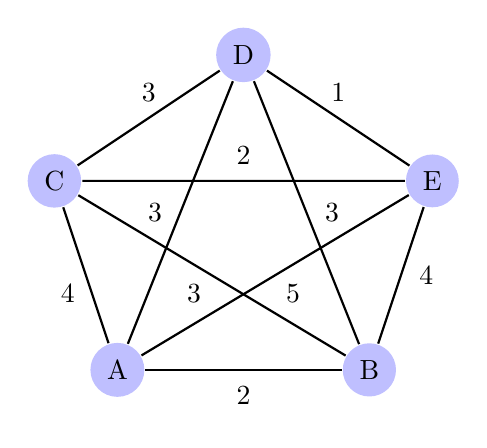
\begin{tikzpicture}
[thick,scale=.8,auto=left,every node/.style={circle,fill=blue!25}]
  \node (na) at (2,0) {A};
  \node (nb) at (6,0) {B};
  \node (nc) at (1,3) {C};
  \node (nd) at (4,5) {D};
  \node (ne) at (7,3) {E};
  \path[-,draw,thick,black]
  	(na) edge node[draw=none,fill=none,below] {$2$} (nb)
  	(nb) edge node[draw=none,fill=none,right] {$4$} (ne)
  	(ne) edge node[draw=none,fill=none,above] {$1$} (nd)
  	(nd) edge node[draw=none,fill=none,above] {$3$} (nc)
  	(nc) edge node[draw=none,fill=none,below left] {$3$} (nb)
  	(na) edge node[draw=none,fill=none] {$4$} (nc)
  	(na) edge node[draw=none,fill=none,below right] {$5$} (ne)
  	(na) edge node[draw=none,fill=none,left] {$3$} (nd)
  	(nd) edge node[draw=none,fill=none,right] {$3$} (nb)
  	(nc) edge node[draw=none,fill=none] {$2$} (ne);
\end{tikzpicture}

  %\path[-,draw,black]
  	%(n3) edge node[draw=none,fill=none] {$e$} (n7);
  %\path[-,draw,very thick,blue,bend right]
  	%(n6) edge node[draw=none,fill=none,color=black] {$e'$} (n7);
  	
  	
 	%\node (n6) at (2,0) {A};
  %\node (n4) at (6,0) {B};
  %\node (n5) at (0,4) {C};
  %\node (n1) at (4,6) {D};
  %\node (n2) at (8,4) {E};
  %\foreach \from/\to in {n6/n5,n4/n2}
    %\draw (\from) -- (\to);